\newpage
\section{Tenacity Paracity}
                                  

In this activity we are going to investigate city geometry parabolas.

\begin{prob} 
Remind me again, what is the definition of a \textit{parabola}?
\end{prob}

\begin{prob}
Use coordinate constructions to find the equation of
the parabola with its focus at $(1,2)$ and its directrix being the line $y=-3$.
\end{prob}



\begin{prob}
Sketch the city geometry parabola when the focus is the point $(0,2)$
and the directrix is $y=0$
\[
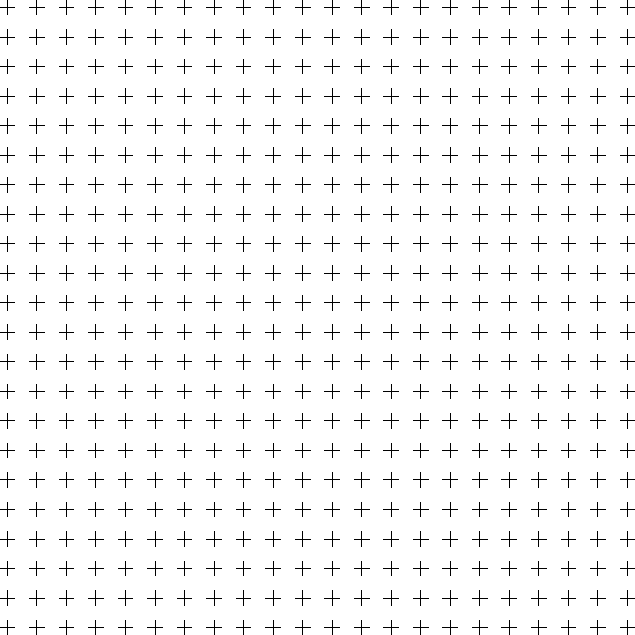
\includegraphics{../graphics/complexPlane}
\]
\end{prob}

\break

\begin{prob}
Sketch the city geometry parabola when the focus is the point $(4,4)$
and the directrix is $y=-x$
\[
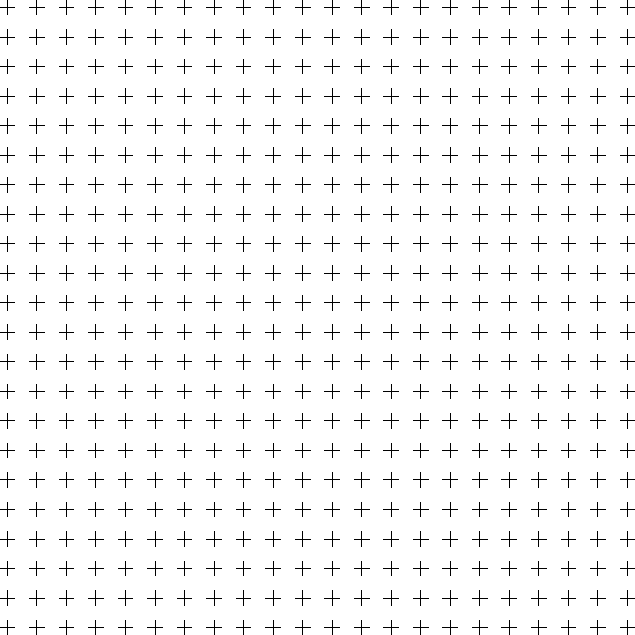
\includegraphics{../graphics/complexPlane}
\]
\end{prob}

\break

\begin{prob}
Sketch the city geometry parabola when the focus is the point $(0,4)$
and the directrix is $y=x/3$
\[
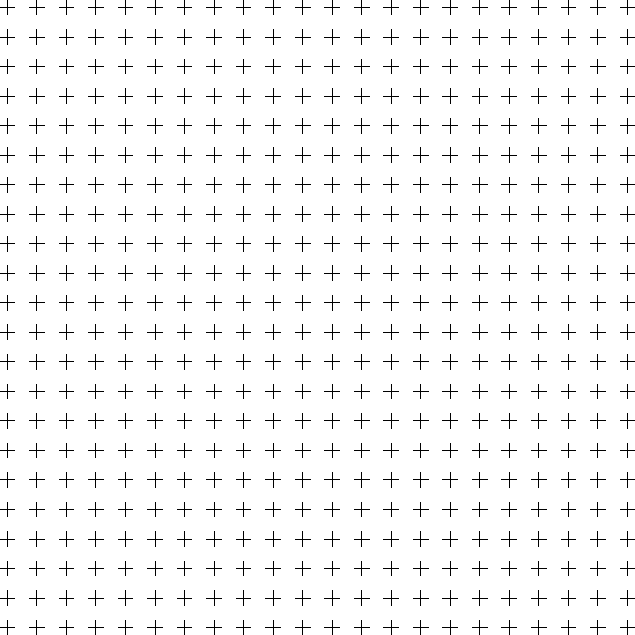
\includegraphics{../graphics/complexPlane}
\]
\end{prob}

\break

\begin{prob}
Sketch the city geometry parabola when the focus is the point $(4,1)$
and the directrix is $y=3x/2$
\[
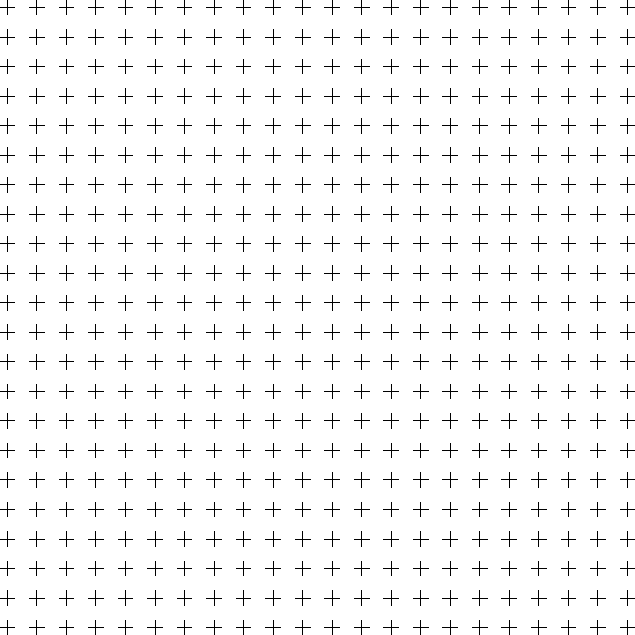
\includegraphics{../graphics/complexPlane}
\]
\end{prob}

\begin{prob}
Explain how to find the distance between a point and a line in city
geometry.
\end{prob}


\begin{prob}
Give instructions for sketching city geometry parabolas.
\end{prob}


